% !Mode:: "TeX:UTF-8"

\chapter{绪论}
\section{课题的研究背景}

人每天接收到的信息里,百分之八十来自于视觉,而这些信息都是以图像的形式进入人的大脑,从而进行处理。可见,图像和人们的密切联系,它是人们认识世界和感受世界的主要媒介。

随着视觉计算和图形学的发展,数字图像处理技术逐渐形成一个独立且完整的理论体系和实现架构。虽然作为一门跨学科的新领域,其发展时间不是很长,但相关技术和应用已经十分完善。尤其是与机器学习和深度学习的结合之后,越来越引起人们的注意。

计算机视觉研究中有不少经典难题,图像分割作为许多不同计算机视觉任务的关键组成部分便是其中一个。
图像分割应用范围十分广泛,例如人脸识别,指纹识别,交通控制系统,在卫星图像中定位物体(道路、森林等),行人检测,医学影像等。

所谓的图像分割根据灰度、彩色、空间纹理、几何形状等特征把图像划分成若干个互不相交的区域,使得这些特征在同一区域内表现出一致性或相似性,而在不同区域间表现出明显的不同。简单的说就是在一副图像中,把目标从背景中分离出来。就是将图像分割成较大的感知区域,每个区域内的像素通常属于同一视觉对象,具有细微的特征差异。它已广泛应用于对象建议生成、目标检测/识别等领域。

与图像分割产生的大的感知区域不同,超像素分割对输入图像进行过分割。它将图像分割成小的、规则的、紧凑的区域,这些区域通常由具有相似空间位置、纹理、颜色、亮度等的像素组成,同时保留了基于像素表示的显著特征。与图像分割相比,超像素通常具有很强的边界相干性,并且产生的分割易于控制。由于超像素在表示和计算方面的高效性,超像素已广泛应用于计算机视觉算法,如对象检测、语义分割、目标跟踪以及显著性估计。

图像分割已有多年的研究历史,分割算法主要分为无监督图像分割和有监督图像分割两大类。无监督分割算法发展较早,已有许多成熟的算法,如聚类、图割、分水岭变换、隐马尔可夫随机场等。这种算法只需要很少的训练样本和标签图像。随着深度学习的发展,有监督的方法,如FCN、U-NET、HFS等,利用CNN网络进行特征学习,实现高效准确的图像分割。有监督学习对数据集的特征进行了更好的编码,使得分割更加精确。

尽管近年来深度学习在计算机视觉中应用更加广泛,但是现有超像素算法如SLIC,WT,是不可微的。并且标准卷积运算通常在规则网格上定义,当在不规则超像素点阵上操作时变得低效。除了一些方法,超像素几乎不与深度网络结合使用。

在本文中,我们提出了一个端到端的可训练网络,使用完全卷积网络和迭代可微聚类算法来获得超像素。
接下来,我们采用超像素池层来获得超像素特征,并以此计算相邻超像素之间的相似度。
如果相似度大于预先设定的阈值,则通过简单的步骤将其合并,得到分割结果。

\begin{figure*}[h]
\centering
\subfigure[原图]{
\begin{minipage}[b]{0.3\linewidth}

\includegraphics[width=1\linewidth]{figures/img/image/176051.jpg}
\end{minipage}}
\hspace{-2.5mm}
\subfigure[图像分割]{
\begin{minipage}[b]{0.3\linewidth}
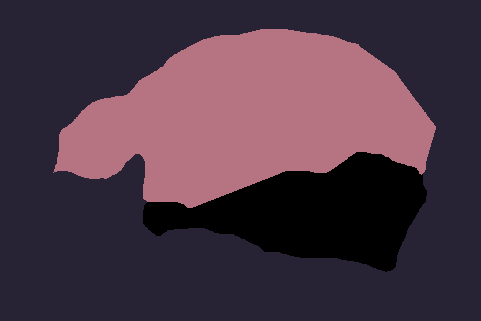
\includegraphics[width=1\linewidth]{figures/img/gt/gt_176051.png}
\end{minipage}}
\hspace{-2.5mm}
\subfigure[超像素分割]{
\begin{minipage}[b]{0.3\linewidth}
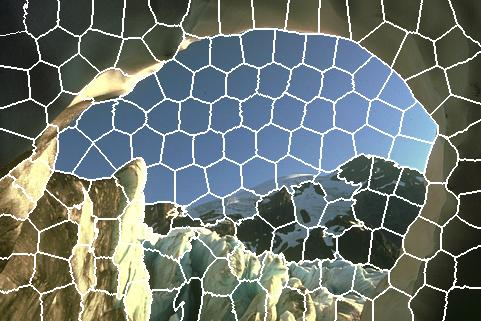
\includegraphics[width=1\linewidth]{figures/img/SLIC/SLIC_176051.jpg}
\end{minipage}}

\caption{图像分割与超像素分割示例}
\end{figure*}

\section{国内外研究现状}

\subsection{超像素分割算法研究现状}

自从Ren和Malik在2003年提出超像素的概念以来,研究人员对这一领域做出了很多贡献,并取得了丰富的成果。
本小结对于超像素算法进行简单整理和介绍。

1. 基于图论法

基于图像法的基本思想是将图像中的像素映射成加权无向图,无向图中的一个顶点代表了图像中的一个像素,点与点之间边的权重由像素之间的特性差异性计算得来。
基于图论法就是将加权无向图根据一定的准则划分为数个连通子树,从而得到超像素分割结果。

设$G=(V,E)$表示由$n$个顶点$v\in V$和$m$个边$e\in E\subseteq V\times V$组成的无向图,每个像素与一个顶点相关联,并与它的4个邻域局部连接。
每个边$e_{ij}=(v_i,v_j)$都被分配了一个权重(通常为非负实值),该权重度量两个顶点之间的差异。
在超像素分割任务中,$k$表示要提取的超像素个数。
超像素分割是将图G划分为k个不相交的分量,每个分量对应一个连通子图${G}'=({V}',{E}')$,
其中${V}'\subseteq V$和${E}'\subseteq E$。

Ncut方法自从提出之后,已经发展了多个版本。它将图像映射到加权无向图中,并定义了目标函数,
包括纹理特征和轮廓特征,通过最小化目标函数,使得分割出的超像素类间距离尽可能大,并且类内距离尽可能小,从而实现超像素分割。虽然它生成的超像素比较规则,但边界的保持效果并不理想,且计算量较大,速度较慢。

2017年,Chen等提出的实现了线性谱聚类(LSC),通过计算像素之间的颜色相似性和空间接近性,利用内核相似度度量函数, 将图像像素巧妙的映射到高维特征空间中, 通过特征空间的加权K-means度量目标函数, 实现低计算量且致密均匀的超像素,大大提升了超像素分割的效率。

2018年,Xing Wei等人提出Superpixel Hierarchy,利用Boruvka 算法实现无向图的区域合并。把一个图看成有n个树的森林(n为图像中像素数目),每个顶点看成一棵树。对于每棵树来说,我们找到它最近的邻点,即边的权重最小的那个点,并把他们合并在一起。Boruvka 算法重复融合树直到只有一棵树留下来。我们用Boruvka 算法生成一个最小生成树(MST),同时记录每个边缘的顺序添加到MST。一旦边缘被添加到MST,森林中的树木数量减少一个。假设需要提取k个超像素,我们通过前n-k个边连接顶点,并且具有k 个连接的组件,这些组件恰好是超像素。

其优点是具有线性时间解,可并行化。此外,该方法在聚类的过程中融入了局部信息,比SLIC和LSC等只利用每像素特征来确定聚类隶属关系的方法更为健壮。

2. 基于梯度下降法

%watersheds,Mean-shift,Quick-shift,Turbopixels,SLIC
简单线性迭代聚类(SLIC)作为最经典的超像素分割算法,具有很多优点,计算简单且速度快,可以生成规则的超像素,此外可以控制超像素数量。但是其生成的超像素边界的保持效果并不理想,而且抗噪性较差。SLIC将彩色图像转换为CIELAB 颜色空间和XY 坐标系下的5维特征向量,然后构造5维特征向量的距离度量来对像素进行局部聚类。这个想法简单易行。与其他超像素分割方法相比,SLIC 算法在速度、紧凑性等方面都是理想的。

zhao等人在SLIC的基础上进行了改进,提出了像素快速线性迭代聚类(FLIC)算法。
FLIC从一个新的角度重新考虑图像的超像素分割问题,利用先验信息,提出了一种名为“Active Search”的新型搜索算法,它明确地考虑了超像素的连通性。
基于这种搜索方法,设计了一个 back-and-forth 的遍历策略并且合并了 SLIC 中的分配和更新步骤。
与 SLIC 相比,SLIC减少了收敛所需的迭代次数,并且提高了超像素分割的边界灵敏度,具有更好的边缘重合度。

3. 基于深度学习的超像素分割算法

近年来,对于广泛的计算机视觉问题采用深度学习的情况急剧增加,但超像素几乎不与现代深度网络结合使用。
这有两个主要原因。首先,标准卷积运算通常定义在规则网格上,当在不规则超像素网格上操作时变得不合适。
其次,现有的超像素算法是不可微的,因此如果在深度网络中使用超像素,
就会在其他端到端可训练网络架构中引入了不可微的模块。

2018年,Varun Jampani等人提出了一种基于深度学习的聚类算法,通过放宽SLIC中存在的最近邻约束将其转化为可微算法。
这种新的可微算法允许端到端训练,从而能够利用强大的深层网络来学习超像素。
其优点包括:端到端可训练,可以轻松集成到其他深层网络架构中;速度快,可以生成边界重合度高的超像素。


\subsection{图像分割研究现状}

(1) 特征空间聚类法

图像分割根据灰度、彩色、空间纹理、几何形状等特征把图像划分成若干个互不相交的区域,
使得这些特征在同一区域内表现出一致性或相似性,而在不同区域间表现出明显的不同。
因此,我们可以将图像分割问题以像素的分类问题来解决。
同类的像素在灰度、彩色、空间纹理等方面具有较高的相似性,而不同类中的像素间差异比较大。

特征空间聚类法作为无监督的图像分割算法,可以减少人为干预,自动完成分割。
但一般需要提前确定分类数,然后通过迭代地来提取各类的特征值,来执行分类算法,
更新聚类中心,例如K-均值,Fuzzy C-means (FCM)聚类算法等。

特征空间聚类作为已经很成熟的算法,有很多优点,例如:不需要训练样本,方法简单,方便执行。
也有相应的缺点:分类数一般很难确定,且初始参数对最终结果有较大的影响。
此外,特征空间聚类没有充分利用像素之间的局部信息,一般只是采用距离或颜色特征,从而对噪声比较敏感。

(2) 边缘检测法

所谓的图像边缘,即在一张图像中,两个不同区域的交界处,图像中相邻区域交界处的像素结果组成了图像的边缘。
根据经验,沿着边缘走向,像素值变化较为平缓;而垂直于边缘,像素值变化较大。
因此,我们可以将图像中灰度发生突变的像素看为边缘。

边缘检测的基本思路一般为:先根据一定的算法来确定图像中的边缘像素集合,目前边缘检测方法来得到边缘像素集合的方法,最实用也最简单方法就是构造边缘算子。采用何种边缘算子来提取图像边缘是边缘检测方法的核心问题。
常见的边缘算子有Roberts,Sobel,PreWitt和Carry等。
边缘检测得到的结果还需要进一步处理,如边缘跟踪,边缘松弛法,将边缘像素连接成图像轮廓,得到图像分割结果。


对于噪声比较小的图像,即图像中的不同区域差别明显,边缘检测方法可以取得较好的结果。若图像比较复杂,且不同区域间的差别不是特别明显,则会产生很多噪声。其难点在于确定边缘时,抗噪性和精确度的矛盾。
若抗噪性提高,就会产生位置偏差或轮廓漏检。若提高边缘精确度,那么噪声就会产生不合理的伪边缘。

(3) 基于区域的方法

类似于边缘检测法,区域分割法利用了图像中局部区域的一致性,直接按照一定的一致性判断来寻找分区,分区内的像素具有相似的性质,最终得到图像分割结果。其中的一致性判断包括:灰度、色彩、纹理、形状等。
基于区域的图像分割大致可以分为两大类:区域生长法,区域分裂与合并。

区域生长法的关键核心在于选取或制定合理的生长准则,按照一定的生长准则将像素或子区域合并成更大的区域。
生长准则可以按照不用的判断标准来制定,基本使用图像的局部信息来制定,如基于灰度级类似准则,基于颜色相似准则,基于纹理相似准则等。
不同的生长准则会影响分割过程,从而对最终的分割结果造成影响。
区域生长法最主要的优点就是计算简单,适合于分割小的结构。但其对噪声敏感,抗噪性弱,导致分区中有空洞。

区域分裂与合并算法的基本思路类似于微分,即无穷分割,然后将分割后满足相似度准则的区域进行合并。
四叉树分解法作为典型的区域分裂合并,应用广泛。我们以灰度级作为分裂合并准则,则基本的分裂与合并算法为:首先对于图像中灰度级不同的区域,均分为4 个子区域;若相邻的子区域所有像素的灰度级相同,则将其合并;重复前面两个步骤,直到不再有新的分裂与合并为止,从而得到最终的分割结果。

区域生长算法和区域分裂合并算法作为基于区域的分割方法,在实际应用中经常结合使用,以取得更好的结果。
该类算法对某些复杂物体定义的复杂场景的分割或者对某些自然景物的分割等类似先验知识不足的图像分割,效果较为理想。

\subsection{利用超像素进行图像分割研究现状}

通过学习像素或超像素的相似性进行分割也是一种趋势。在(Ahn and Kwak,2018)中,作者提出了仿射网来预测一对相邻图像坐标之间的语义一致性。利用仿射网预测的邻接词,通过随机游动实现语义传播。基于超像素描述子向量之间的距离度量来计算超像素相似度,(Chaibou et al.,2020)引入了一种新的超像素上下文描述器来增强学习特征,以更好地进行相似性预测。然后通过迭代合并使用相似性加权目标函数选择的最相似的超像素对来实现图像分割。

超像素池网络(SPN)提出的超像素池为超像素特征提取提供了新思路。SPN利用输入图像的超像素分割作为一个池布局来反映底层图像结构,用于学习和推断语义分割。由SPN生成的初始注释被用来学习另一个神经网络来估计像素语义标签。DEL算法利用超像素池运算提取超像素特征进行图像分割,取得了良好的效果。在提取的超像素的基础上,利用超像素池运算提取超像素的特征来计算超像素的相似度。根据相似度来判断超像素是否进行合并,从而得到最终的分割结果。

2018年,Tao Lei等人提出了SFFCM,其算法通过多尺度形态梯度重建(MMGR)和分水岭变换(WT)获得超像素,然后利用基于超像素的SFFCM进行图像分割。
与其他聚类算法相比,该算法耗时更少。然而,聚类中心的初始值难以确定,不能得到广泛的应用。


\section{论文研究内容和结构安排}

\subsection{论文研究内容}

本文的主要研究内容是计算机视觉中两个主要的方向-超像素分割,图像分割。虽然现在有很多优秀且成熟的算法来实现超像素分割或者图像分割,但也存在一些问题:首先现在的神经网络没有将超像素分割和图像分割两个任务有效的结合起来,只有部分算法将现有的超像素作为图像分割的输入进行计算。其次,现有的超像素算法基本还是以传统算法为主,并没有真正与神经网络结合起来,发挥神经网络的优势。此外,图像分割算法还是基本以像素为单位进行运算,并没有引入超像素进入有效的计算。

针对此问题,本文提出了端到端的可训练网络,可以同时产生超像素和进行图像分割。
使用完全卷积网络和迭代可微聚类算法来获得超像素。
接下来,采用超像素池层来获得超像素特征,并以此计算相邻超像素之间的相似度。
如果相似度大于预先设定的阈值,则通过简单的步骤将其合并,得到目标片段。
本文在使用BSDS500数据集上,最先进的结果进行多次使用比较,结果验证了本文方法的有效性和可行性,
实现了精细的超像素分割和图像分割。

\subsection{论文结构安排}

本文结构安排如下:

第1章为绪论,介绍了超像素和图像分割的基本概念,并分类介绍了超像素分割和图像分割的经典方法,
最后简要介绍了本文。

第2章首先简介了深度学习和神经网络理论,然后详细介绍了卷积神经网络基本理论,并简单介绍了超像素池化方法。

第3章首先回顾了经典的SLIC方法的核心步骤,然后介绍了对SLIC 的改进,并利用提出的损失函数进行超像素分割。

第4章介绍了在第3章产生超像素的基础上,进行计算超像素相似度以及超像素融合步骤。

第5章首先说明本文使用的实验环境及对比介绍本文使用的深度学习框架,其次介绍本文实验中的公开数据集及评定标准;最后对本文介绍的网络模型以及改进的网络模型进行实验及对比分析。

第6章对全文进行总结,并对未来基于卷积神经网络的图像分割和超像素分割方法的发展进行了展望。 